\subsection{Diagramma di flusso}
Per comprendere meglio il processo dell’algoritmo viene mostrato il diagramma di flusso in \figurename~\ref{fig:flowchart}, nel quale viene mostrato il flusso di un ordine dal momento in cui viene effettuato dal cliente a quando viene assegnato alla postazione di lavoro in cucina.
\begin{figure}[htbp]
	\centering
	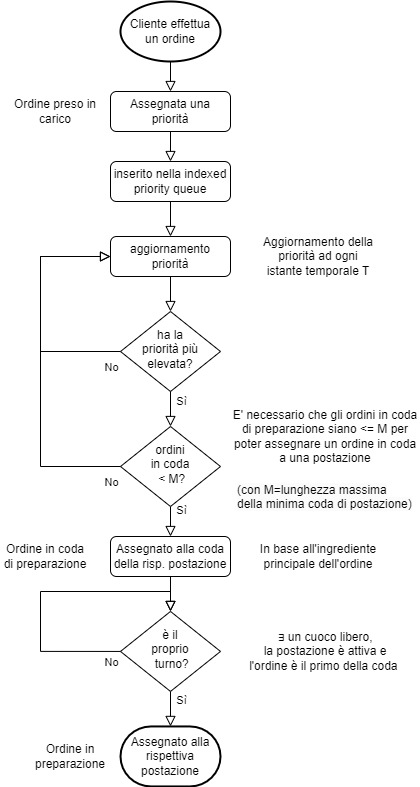
\includegraphics[scale=0.6]{iterazione2/images/flowchart.jpg}
	\caption{Diagramma di flusso\label{fig:flowchart}}
\end{figure}

\clearpage